\documentclass[reprint,amsmath,amssymb,aps,floatfix]{revtex4-2}
\usepackage{balance}
\usepackage[%
    margin=10mm,% ако не си принтира 10мм не изглежда грозно, а може да събереш повече текст
    % showframe=true,%
    ]{geometry}
\usepackage[T1,T2A]{fontenc}
\usepackage[utf8]{inputenc}
\usepackage[main=bulgarian, english]{babel}
\usepackage{float}
\AtBeginDocument{\selectlanguage{bulgarian}}
\newcommand{\degree}{^{\circ}}
\usepackage{amsmath}
\usepackage{graphics}
\usepackage{graphicx}
\graphicspath{{.}}
\usepackage{booktabs} % от тук се използва само \midrule може и без него 
\usepackage{dcolumn}
\usepackage{lipsum}
\newcolumntype{d}[1]{D{.}{.}{#1}}
\usepackage[unicode=true,pdfusetitle]{hyperref}
\usepackage[]{siunitx}
% \usepackage{balance}


\usepackage[compact]{titlesec}

\begin{document}

\title{Повърхностно напрежение на смеси от спирт и вода}

\author{Васил Николов}
\date{26.04.2022}
\maketitle

\section{Цел на упражнението}

Да се определи по абсолютен и относителен метод коефициентът на повърхностно напрежение на смеси от вода и етилов спирт. 

\section{Експериментална установка}

Експериментална установка се състои от капилярка, чийто долен ръб докосва изследваната течност, а отгове е отворена към атвосферата. Течността е в затворен съд, като към капачката му е свързана и тръба, другият край на която е свързана към манометър, и налягането може да се изменя ????? . В експеримента се мери налягането, при което през капиляркакта започват да се отделят балончета. 

\section{Теоретична обосновка}
\subsection{Абсолютен метод}

Тъй като водата и спиртът мокри капилярката кривината на менискуса ще създаде отрицателно налягане, и течността ще се покачи нагоре. Нека покачването на сместа в капиляркатата е $\Delta h$, налягането в съда е $P$, плътността на сместа е $\rho$. Плътността на водата в манометъра е $\rho_w$, а неговото ниво се променя с $\Delta H_m$. Тогава 
\begin{gather*}
    P_{atm} - \frac{2\sigma}{R} + \rho g \Delta H = P \\
    \frac{2\sigma}{R} = P_{atm} - P + \rho g \Delta H \\
    \sigma = (P_{atm} - P)\frac{R}{2} = \frac{\rho_w g \Delta H_m R}{2} \label{eq:1} \tag{1}
\end{gather*}

В последното уравнение \eqref{eq:1} използваме, че правим измерване когато започнат да се появяват балончета от капилярката, тоест покачването на нивото на сместа в нея $\Delta H = 0$. 

За да намерим неизвестната концентрация $X$ ще фитираме крива на експерименталните данни и ще интерполираме. 

\subsection{Относителен метод}

При относителният метод измерванията са същите, но вместо да смятаме директно повърхностното напрежение по \eqref{eq:1} първо калибрираме уреда. Знаейки добре повърхностното напрежение на водата $\sigma_w = 72.75 \ \si{J m^{-2}}$. Въвеждаме константа $B$, и чрез нея ще пресмятаме повърхностните напрежения на смесите. 

\begin{gather*}
    B = \frac{\sigma_w}{\Delta H_w} \\
    \sigma_x = B \Delta H_x \label{eq:2} \tag{2}
\end{gather*}

От данните за дестилираната вода пресмятаме числената стойност на $B = 1.35 \ \si{Jm^{-3}} \pm 3\% $. 
По уравнение \eqref{eq:2} можем да пресмятаме повърхностните напрежения на различните смеси. Тъй като обаче параметрите на установката не се променят, то можем да запишем следната връзка между коефициентите, сметнати по абсолютния и остносителния метод

\begin{equation*}
    \sigma_R = \frac{2B}{\rho_w g R} \sigma_A \label{eq:3} \approx 0.98 \sigma_A  \tag{3}
\end{equation*}

\section{Експериментални данни и резултати}
\subsection{Абсолютен метод}

По описаният горе абсолютен метод пресмятаме коефициентите на повърхностно напрежение на смесите. Неточностите на пресмятанията са около $3\%$. Резултатите са представени на Фигура 1 

\begin{figure}[H] \label{fig:1} 
    \centering
    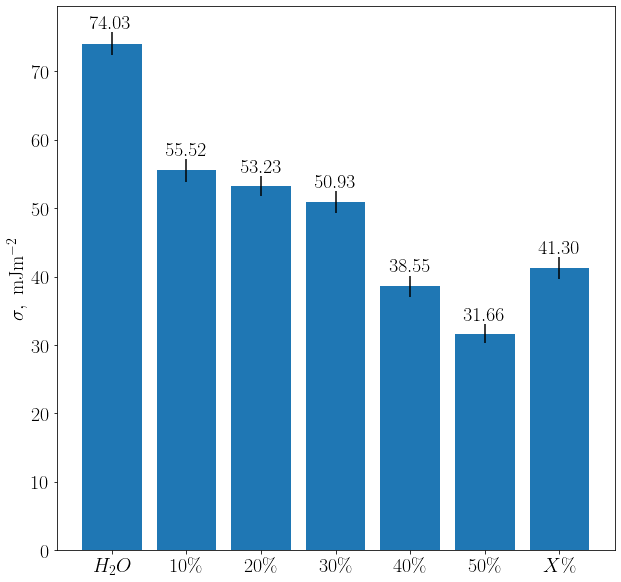
\includegraphics[width=0.9\columnwidth, keepaspectratio=true]{absolute.png}
    \caption{Коефициенти на повърхностно напрежение, абсолютен метод}
\end{figure}

След като фитираме полином от 3та степен на данните и интерполираме получаваме, че неизвестната концентрация $c_x = (41.3 \pm 2)\%$
\subsection{Относителен метод}

Заради уравнение \eqref{eq:3} коефициентите, получени по относителният метод са пропорционални на тези, получени по абсолютният. Аналогично, отново ще получим същата стойност за неизвестната концентрация. 

\end{document}

